%% abtex2-modelo-trabalho-academico.tex, v-1.9.6 laurocesar
%% Copyright 2012-2016 by abnTeX2 group at http://www.abntex.net.br/ 
%%
%% This work may be distributed and/or modified under the
%% conditions of the LaTeX Project Public License, either version 1.3
%% of this license or (at your option) any later version.
%% The latest version of this license is in
%%   http://www.latex-project.org/lppl.txt
%% and version 1.3 or later is part of all distributions of LaTeX
%% version 2005/12/01 or later.
%%
%% This work has the LPPL maintenance status `maintained'.
%% 
%% The Current Maintainer of this work is the abnTeX2 team, led
%% by Lauro César Araujo. Further information are available on 
%% http://www.abntex.net.br/
%%
%% This work consists of the files abntex2-modelo-trabalho-academico.tex,
%% abntex2-modelo-include-comandos and abntex2-modelo-references.bib
%%

% ------------------------------------------------------------------------
% ------------------------------------------------------------------------
% abnTeX2: Modelo de Trabalho Academico (tese de doutorado, dissertacao de
% mestrado e trabalhos monograficos em geral) em conformidade com 
% ABNT NBR 14724:2011: Informacao e documentacao - Trabalhos academicos -
% Apresentacao
% ------------------------------------------------------------------------
% ------------------------------------------------------------------------

\documentclass[
	% -- opções da classe memoir --
	12pt,				% tamanho da fonte
	%openright,			% capítulos começam em pág ímpar (insere página vazia caso preciso)
	%twoside,			% para impressão em recto e verso. Oposto a oneside
	oneside,			% impressão de um lado só
	a4paper,			% tamanho do papel. 
	% -- opções da classe abntex2 --
	chapter=TITLE,		% títulos de capítulos convertidos em letras maiúsculas
	section=TITLE,		% títulos de seções convertidos em letras maiúsculas
	%subsection=TITLE,	% títulos de subseções convertidos em letras maiúsculas
	%subsubsection=TITLE,% títulos de subsubseções convertidos em letras maiúsculas
	sumario=tradicional % opção de sumário
	% -- opções do pacote babel --
	english,			% idioma adicional para hifenização
	french,				% idioma adicional para hifenização
	spanish,			% idioma adicional para hifenização
	brazil				% o último idioma é o principal do documento
	]{abntex2}

% ---
% Pacotes básicos 
% ---
\usepackage{lmodern}			% Usa a fonte Latin Modern			
\usepackage[T1]{fontenc}		% Selecao de codigos de fonte.
\usepackage[utf8]{inputenc}		% Codificacao do documento (conversão automática dos acentos)
\usepackage{lastpage}			% Usado pela Ficha catalográfica
\usepackage{indentfirst}		% Indenta o primeiro parágrafo de cada seção.
\usepackage{color}				% Controle das cores
\usepackage{graphicx}			% Inclusão de gráficos
\usepackage{microtype} 			% Melhorias de justificação
\usepackage{hyperref}
\usepackage{facens}				% Padrão Facens
\usepackage{pdfpages}			% Include de pdfs
\usepackage{lipsum}				% Geração de dummy text
\usepackage[alf]{abntex2cite}	% Citações padrão ABNT
%\usepackage[brazilian,hyperpageref]{backref}	 % Paginas com as citações na bibl
% ---

% ---
% Indicando pasta de figuras\\
% ---
\graphicspath{{imagens/}}
% ---

% --- 
% CONFIGURAÇÕES DE PACOTES
% --- 

% ---
% Configurações do pacote backref
% Usado sem a opção hyperpageref de backref
%\renewcommand{\backrefpagesname}{Citado na(s) página(s):~}
% Texto padrão antes do número das páginas
%\renewcommand{\backref}{}
% Define os textos da citação
%\renewcommand*{\backrefalt}[4]{
%	\ifcase #1 %
%		Nenhuma citação no texto.%
%	\or
%		Citado na página #2.%
%	\else
%		Citado #1 vezes nas páginas #2.%
%	\fi}%
% ---

%VARIAVEIS
%---

%---
% ---
% Informações de dados para CAPA e FOLHA DE ROSTO
% ---
\titulo{RELATÓRIO DE ESTÁGIO SUPERVISIONADO OBRIGATÓRIO}
\autor{Alex Covolan Vieira Coelho}
\local{Sorocaba/SP}
\data{2017}
\orientador[Dra.]{Andrea Vieira Braga}
\instituicao{Faculdade de Engenharia de Sorocaba - FACENS}
\tipotrabalho{Dissertação}

% O preambulo deve conter o tipo do trabalho, o objetivo, 
% o nome da instituição e a área de concentração 
\preambulo{Relatório apresentado como requisito obrigatório para a integralização do Curso de Engenharia da Computação.}
% ---


% ---
% Configurações de aparência do PDF final

% alterando o aspecto da cor azul
\definecolor{blue}{RGB}{41,5,195}

% informações do PDF
\makeatletter
\hypersetup{
     	%pagebackref=true,
		pdftitle={\@title}, 
		pdfauthor={\@author},
    	pdfsubject={\imprimirpreambulo},
	    pdfcreator={LaTeX with abnTeX2},
		pdfkeywords={abnt}{latex}{abntex}{abntex2}{trabalho acadêmico}, 
		colorlinks=false,       		% false: boxed links; true: colored links
    	linkcolor=blue,          	% color of internal links
    	citecolor=blue,        		% color of links to bibliography
    	filecolor=magenta,      		% color of file links
		urlcolor=blue,
		bookmarksdepth=4
}
\makeatother
% --- 

% --- 
% Espaçamentos entre linhas e parágrafos 
% --- 

% O tamanho do parágrafo é dado por:
\setlength{\parindent}{1.25cm}

% Controle do espaçamento entre um parágrafo e outro:
\setlength{\parskip}{0.2cm}  % tente também \onelineskip

% ---
% compila o indice
% ---
\makeindex
% ---

% ----
% Início do documento
% ----
\begin{document}
% Seleciona o idioma do documento (conforme pacotes do babel)
%\selectlanguage{english}
\selectlanguage{brazil}

% Retira espaço extra obsoleto entre as frases.
\frenchspacing 

% ----------------------------------------------------------
% ELEMENTOS PRÉ-TEXTUAIS
% ----------------------------------------------------------
\pretextual

%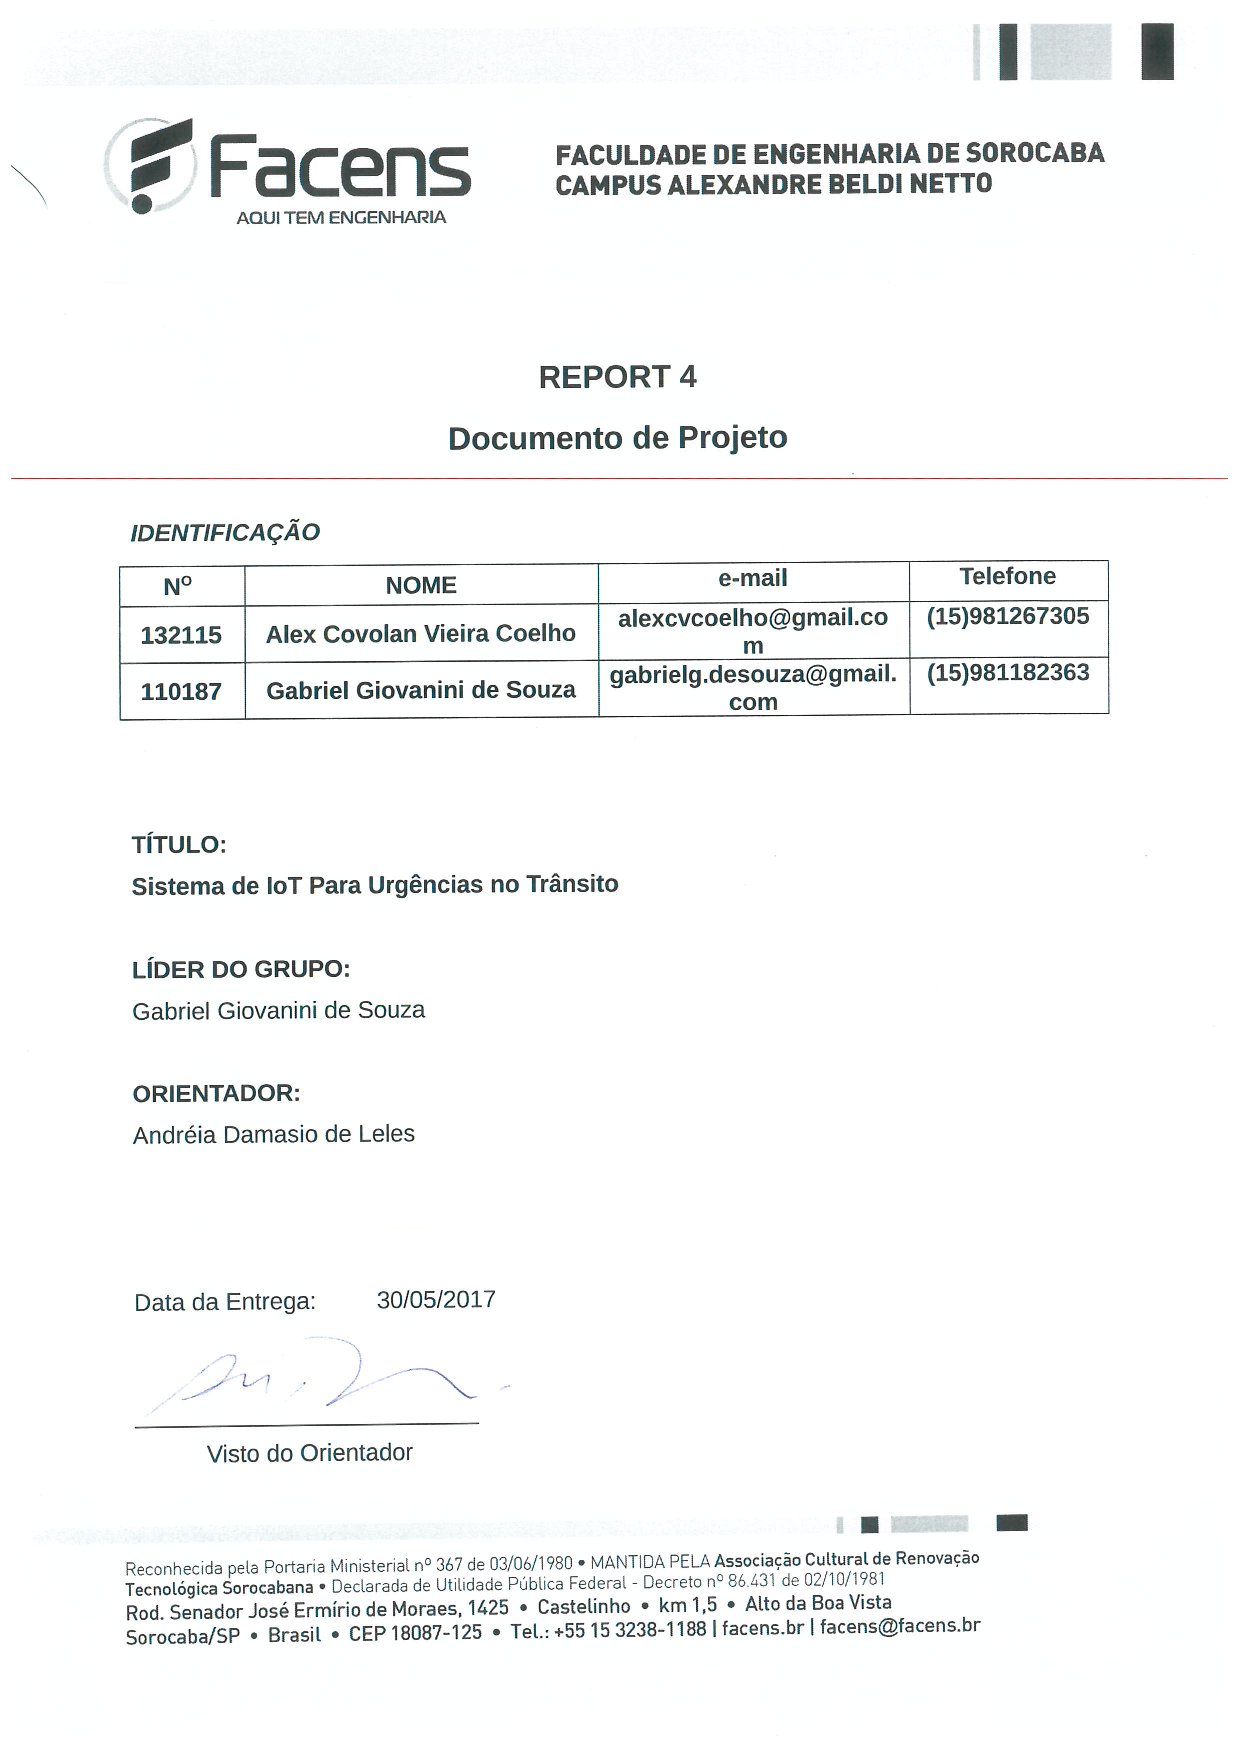
\includepdf{report4.pdf}


% ---
% Capa
% ---
\imprimircapa
% ---

% ---
% Folha de rosto
% (o * indica que haverá a ficha bibliográfica)
% ---
\imprimirfolhaderosto*
% ---

% ---
% Inserir a ficha bibliografica
% ---

% Isto é um exemplo de Ficha Catalográfica, ou ``Dados internacionais de
% catalogação-na-publicação''. Você pode utilizar este modelo como referência. 
% Porém, provavelmente a biblioteca da sua universidade lhe fornecerá um PDF
% com a ficha catalográfica definitiva após a defesa do trabalho. Quando estiver
% com o documento, salve-o como PDF no diretório do seu projeto e substitua todo
% o conteúdo de implementação deste arquivo pelo comando abaixo:
%
% \begin{fichacatalografica}
%     \includepdf{fig_ficha_catalografica.pdf}
% \end{fichacatalografica}

%\begin{fichacatalografica}
	\sffamily
	\vspace*{\fill}					% Posição vertical
	\begin{center}					% Minipage Centralizado
	\fbox{\begin{minipage}[c][8cm]{13.5cm}		% Largura
	\small
	\imprimirautor
	%Sobrenome, Nome do autor
	
	\hspace{0.5cm} \imprimirtitulo  / \imprimirautor. --
	\imprimirlocal, \imprimirdata-
	
	\hspace{0.5cm} \pageref{LastPage} p. : il. (algumas color.) ; 30 cm.\\
	
	\hspace{0.5cm} \imprimirorientadorRotulo~\imprimirorientador\\
	
	\hspace{0.5cm}
	\parbox[t]{\textwidth}{\imprimirtipotrabalho~--~\imprimirinstituicao,
	\imprimirdata.}\\
	
	\hspace{0.5cm}
		1. Palavra-chave1.
		2. Palavra-chave2.
		2. Palavra-chave3.
		I. Orientador.
		II. Universidade xxx.
		III. Faculdade de xxx.
		IV. Título 			
	\end{minipage}}
	\end{center}
\end{fichacatalografica}
% ---

% ---
% Inserir errata
% ---
%\begin{errata}
Elemento opcional da \citeonline[4.2.1.2]{NBR14724:2011}. Exemplo:

\vspace{\onelineskip}

FERRIGNO, C. R. A. \textbf{Tratamento de neoplasias ósseas apendiculares com
reimplantação de enxerto ósseo autólogo autoclavado associado ao plasma
rico em plaquetas}: estudo crítico na cirurgia de preservação de membro em
cães. 2011. 128 f. Tese (Livre-Docência) - Faculdade de Medicina Veterinária e
Zootecnia, Universidade de São Paulo, São Paulo, 2011.

\begin{table}[htb]
\center
\footnotesize
\begin{tabular}{|p{1.4cm}|p{1cm}|p{3cm}|p{3cm}|}
  \hline
   \textbf{Folha} & \textbf{Linha}  & \textbf{Onde se lê}  & \textbf{Leia-se}  \\
    \hline
    1 & 10 & auto-conclavo & autoconclavo\\
   \hline
\end{tabular}
\end{table}

\end{errata}
% ---

% ---
% Inserir folha de aprovação
% ---

% Isto é um exemplo de Folha de aprovação, elemento obrigatório da NBR
% 14724/2011 (seção 4.2.1.3). Você pode utilizar este modelo até a aprovação
% do trabalho. Após isso, substitua todo o conteúdo deste arquivo por uma
% imagem da página assinada pela banca com o comando abaixo:
%
% \includepdf{folhadeaprovacao_final.pdf}
%
%\begin{folhadeaprovacao}

  \begin{center}
    {\ABNTEXchapterfont\large\imprimirautor}

    \vspace*{\fill}\vspace*{\fill}
    \begin{center}
      \ABNTEXchapterfont\bfseries\Large\imprimirtitulo
    \end{center}
    \vspace*{\fill}
    
    \hspace{.45\textwidth}
    \begin{minipage}{.5\textwidth}
        \imprimirpreambulo
    \end{minipage}%
    \vspace*{\fill}
   \end{center}
        
   Trabalho aprovado. \imprimirlocal, 24 de novembro de 2012:

   \assinatura{\textbf{\imprimirorientador} \\ Orientador} 
   \assinatura{\textbf{Professor} \\ Convidado 1}
   \assinatura{\textbf{Professor} \\ Convidado 2}
   %\assinatura{\textbf{Professor} \\ Convidado 3}
   %\assinatura{\textbf{Professor} \\ Convidado 4}
      
   \begin{center}
    \vspace*{0.5cm}
    {\large\imprimirlocal}
    \par
    {\large\imprimirdata}
    \vspace*{1cm}
  \end{center}
  
\end{folhadeaprovacao}
% ---

% ---
% Dedicatória
% ---
%\begin{dedicatoria}
   \vspace*{\fill}
   \centering
   \noindent
   \textit{ Este trabalho é dedicado às crianças adultas que,\\
   quando pequenas, sonharam em se tornar cientistas.} \vspace*{\fill}
\end{dedicatoria}
% ---

% ---
% Agradecimentos
% ---
%\begin{agradecimentos}
Os agradecimentos principais são direcionados à Gerald Weber, Miguel Frasson,
Leslie H. Watter, Bruno Parente Lima, Flávio de Vasconcellos Corrêa, Otavio Real
Salvador, Renato Machnievscz\footnote{Os nomes dos integrantes do primeiro
projeto abn\TeX\ foram extraídos de
\url{http://codigolivre.org.br/projects/abntex/}} e todos aqueles que
contribuíram para que a produção de trabalhos acadêmicos conforme
as normas ABNT com \LaTeX\ fosse possível.

Agradecimentos especiais são direcionados ao Centro de Pesquisa em Arquitetura
da Informação\footnote{\url{http://www.cpai.unb.br/}} da Universidade de
Brasília (CPAI), ao grupo de usuários
\emph{latex-br}\footnote{\url{http://groups.google.com/group/latex-br}} e aos
novos voluntários do grupo
\emph{\abnTeX}\footnote{\url{http://groups.google.com/group/abntex2} e
\url{http://www.abntex.net.br/}}~que contribuíram e que ainda
contribuirão para a evolução do \abnTeX.

\end{agradecimentos}
% ---

% ---
% Epígrafe
% ---
%\begin{epigrafe}
    \vspace*{\fill}
	\begin{flushright}
		\textit{``Não vos amoldeis às estruturas deste mundo, \\
		mas transformai-vos pela renovação da mente, \\
		a fim de distinguir qual é a vontade de Deus: \\
		o que é bom, o que Lhe é agradável, o que é perfeito.\\
		(Bíblia Sagrada, Romanos 12, 2)}
	\end{flushright}
\end{epigrafe}
% ---

% ---
% RESUMOS
% ---

% resumo em português
%\setlength{\absparsep}{18pt} % ajusta o espaçamento dos parágrafos do resumo
\begin{resumo}
 Segundo a \citeonline[3.1-3.2]{NBR6028:2003}, o resumo deve ressaltar o
 objetivo, o método, os resultados e as conclusões do documento. A ordem e a extensão
 destes itens dependem do tipo de resumo (informativo ou indicativo) e do
 tratamento que cada item recebe no documento original. O resumo deve ser
 precedido da referência do documento, com exceção do resumo inserido no
 próprio documento. (\ldots) As palavras-chave devem figurar logo abaixo do
 resumo, antecedidas da expressão Palavras-chave:, separadas entre si por
 ponto e finalizadas também por ponto.

 \textbf{Palavras-chave}: latex. abntex. editoração de texto.
\end{resumo}

% resumo em inglês
%\begin{resumo}[Abstract]
 \begin{otherlanguage*}{english}
   This is the english abstract.

   \vspace{\onelineskip}
 
   \noindent 
   \textbf{Keywords}: latex. abntex. text editoration.
 \end{otherlanguage*}
\end{resumo}

% ---

% ---
% inserir lista de ilustrações
% ---
\pdfbookmark[0]{\listfigurename}{lof}
\listoffigures*
\cleardoublepage
% ---

% ---
% inserir lista de tabelas
% ---
%\pdfbookmark[0]{\listtablename}{lot}
\listoftables*
\cleardoublepage
% ---

% ---
% inserir lista de abreviaturas e siglas
% ---
%\begin{siglas}
  \item[CRTSE] Centro Regional de Tecnologia Santa Escolástica
  \item[CRTS] Companhia Rede Telefônica Sorocabana
  \item[ACRTS] Associação Cultural de Renovação Tecnológica Sorocabana
  \item[IPEAS] Instituto de Pesquisas e Estudos Avançados Sorocabano
  \item[LEMAT] Laboratório de Ensaio de Materiais
  \item[ABMES] Associação Brasileira de Mantenedoras de Ensino Superior
\end{siglas}
% ---

% ---
% inserir lista de símbolos
% ---
%\begin{simbolos}
  \item[$ \Gamma $] Letra grega Gama
  \item[$ \Lambda $] Lambda
  \item[$ \zeta $] Letra grega minúscula zeta
  \item[$ \in $] Pertence
\end{simbolos}
% ---

% ---
% inserir o sumario
% ---
\pdfbookmark[0]{\contentsname}{toc}
\tableofcontents*
\cleardoublepage
% ---



% ----------------------------------------------------------
% ELEMENTOS TEXTUAIS
% ----------------------------------------------------------
\textual
% ---
\pagestyle{simple}


\chapter{Introdução}
\label{chap:cap1}
O presente relatório de estágio é elaborado como documento obrigatório para a conclusão do curso de Engenharia da Computação, apresentando as atividades realizadas durante as 360 horas de estágio, cumpridas dentro da Faculdade de Engenharia de Sorocaba (Facens). Mais especificamente atuando dentro do Laboratório de Informática, nos primeiros meses trabalhando com suporte aos computadores presentes na faculdade, além de atendimento \textit{help desk} e posteriormente trabalhando com desenvolvimento de aplicações WEB em PHP as quais serviram para atender as demandas da própria faculdade, tanto no âmbito corporativo como no educacional.

Tal estágio também proporcionou uma posterior contratação ao término dos 2 anos previsto em contrato, e este é o período considerado neste documento, pois após a contratação as áreas de atuação foram ampliadas, garantindo sólidos conhecimentos em novas tecnologias e plataformas, como Ruby, C\# e a plataforma Sales Force, compreendendo o período de maior aprendizado durante esta jornada. 

Mesmo com as novas tecnologias e áreas de atuação, a maior parte das aplicações a serem criadas continuaram sendo em PHP, além de dar suporte as aplicações antigas. Foi possível também aprender sobre a área de infraestrutura, passando a desempenhar a função de \textit{devops} e trabalhando ao lado dos analistas de redes.

Dentre os feitos durante o estágio, destaca-se a doação de um sistema de inscrições para a FUNDEC (Fundação de Desenvolvimento Cultural de Sorocaba), tal sistema agilizou a inscrição e processo de seleção de mais de 4 mil candidatos, os quais eram cadastrados na mão anteriormente, também é possível enunciar a colaboração no desenvolvimento de uma \textit{framework} própria desenvolvida dentro da FACENS pelo Eng. Flávio Bogila a qual ganhou o nome de "Bogila Framework", através dela possibilitou-se criar novas aplicações com maior velocidade devido ao fato dela já possuir \textit{templates} padrões, geração de código e uma arquitetura que facilitam seu uso nas aplicações da Faculdade.

\chapter{Plano de Estágio}
\label{chap:cap2}
Informações sobre a empresa e o estagiário são apresentados nesta seção.
\section{Identificação do Aluno}
\label{sec:identaluno}
\textbf{Nome:} Alex Covolan Vieira Coelho\\
\indent \textbf{Matrícula: } 132115\\
\indent \textbf{Curso: } Engenharia da Computação\\
\indent \textbf{Semestre: } 10º\\
\indent \textbf{Ano de ingresso: } 2013\\
\indent \textbf{E-mail: } alexcvcoelho@gmail.com\\

\section{Empresa}
\label{sec:empresa}
\textbf{Nome:} FACENS - Faculdade de Engenharia de Sorocaba \\
\indent \textbf{Razão Social:} Associacao Cultural de Renovacao Tecnologica Sorocabana \\
\indent \textbf{CNPJ:} 45.718.988/0003-29 \\
\indent \textbf{Área de atuação:} Educação superior\\
\indent \textbf{Endereço:} Rodovia Senador José Ermírio de Moraes, 1425 \\
\indent \textbf{Bairro:} Castelinho km 1,5 - Alto da Boa Vista \\
\indent \textbf{CEP:} 18087-125 \\
\indent \textbf{Cidade:} Sorocaba \\
\indent \textbf{Estado:} São Paulo \\
\indent \textbf{Nome do responsável pelos estágios na empresa:} João Alex Ramon \\
\indent \textbf{Telefone da área responsável pelos estágios:} (15) 3238-1188/216 \\

\begin{figure}[htb]
\caption{\label{fig:mapsfacens} Localização da Facens}
\begin{center}
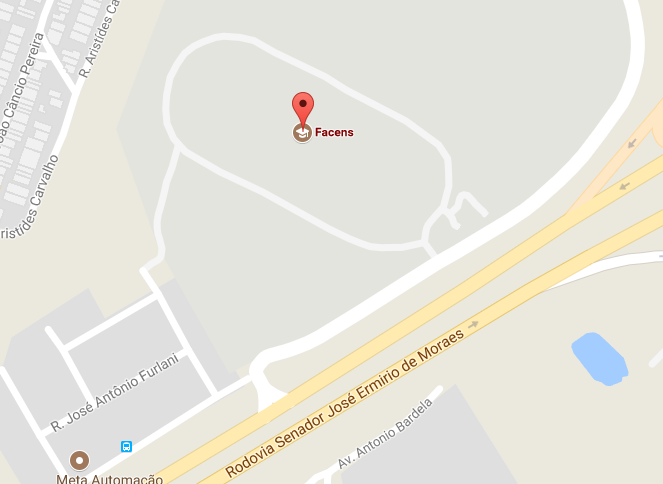
\includegraphics[scale=0.65]{MapsFacens}
\end{center}
\end{figure}

\section{Estágio}
\label{sec:estagio}
\textbf{Área de atuação:} Desenvolvimento \\
\indent \textbf{Setor:} TI \\
\indent \textbf{Data de início de estágio:} \\
\indent \textbf{Data do fim de estágio:} \\
\indent \textbf{Período do dia que estagia:} Manhã e Tarde \\
\indent \textbf{Carga horária semanal:} 40 horas \\

\section{Supervisor de Estágio na Empresa}
\label{sec:supestagioempre}
\textbf{Nome:} Luis Gustavo Martins Monteiro \\
\indent \textbf{Formação acadêmica:} \\
\indent \indent Especialização em Redes de Computadores, UNICAMP, 2006 \\
\indent \indent Graduação em Sistemas de Informação, Uirapuru Superior, 2005 \\
\indent \textbf{Cargo:} Coordenador da Tecnologia da Informação \\
\indent \textbf{Departamento:} TI \\
\indent \textbf{Responsabilidades do departamento:} Desenvolvimento e suporte de soluções tecnológicas \\
\indent \textbf{Telefone:} (15) 3238-1188/236 \\
\indent \textbf{E-mail:} gustavo.monteiro@facens.br \\

\section{Atividades Programadas Para o Estagiário}
\label{sec:ativestagiario}


\chapter{Organograma da Empresa}
\label{chap:chap3}
\textbf{Diretor:} \\ \indent Eng. Paulo Roberto Freitas de Carvalho \\
\indent paulo.carvalho@facens.br \\

\textbf{Vice Diretor:} \\ \indent  Prof. Dr. Fabiano Prado Marques \\
\indent fabiano.marques@facens.br \\

\textbf{Coordenação Engenharia Civil:}\\ \indent  Prof. Dr. José Antonio De Milito \\
\indent jose.milito@facens.br \\

\textbf{Coordenação Engenharia da Computação:}\\ \indent Prof.ª Dra. Andréa Lucia Braga Vieira Rodrigues \\
\indent andrea.braga@facens.br \\

\textbf{Coordenação Engenharia Elétrica:} \\ \indent Prof. Dr. Anderson Marcos Henriques \\
\indent anderson.henriques@facens.br \\

\textbf{Coordenação Engenharia Mecânica:} \\ \indent Prof. Dr. Francisco Scinocca \\
\indent francisco.scinocca@facens.br \\

\textbf{Coordenação Engenharia Mecatrônica:} \\ \indent Prof. Dr. Anderson Marcos Henriques \\
\indent anderson.henriques@facens.br \\

\textbf{Coordenação Engenharia Produção:} \\ \indent Prof. Dr. José Lázaro Ferraz \\
\indent jose.ferraz@facens.br \\

\textbf{Coordenação Engenharia Química:} \\ \indent Prof.ª Dra. Sandra Bizarria Lopes Villanueva \\
\indent sandra.lopes@facens.br \\

\textbf{Coordenação Tecnologia em Jogos Digitais:} \\ \indent Prof.ª Dra. Andréa Lucia Braga Vieira Rodrigues \\
\indent andrea.braga@facens.br \\

\textbf{Coordenação Engenharia Agronômica:} \\ \indent Prof.ª Me. Thais Prado Avancini \\
\indent thais.avancini@facens.br \\

\textbf{Coordenação Engenharia de Alimentos:} \\ \indent Prof. Dra. Cláudia Maria Treumann Rocha \\
\indent claudia.treumann@facens.br \\

\textbf{Coordenação Acadêmica:} \\ \indent Prof.ª Dra. Sandra Bizarria Lopes Villanueva \\
\indent sandra.lopes@facens.br \\

\textbf{Coordenação Ciclo Básico:} \\ \indent Prof. Me. Marcos Vinícius Ribeiro \\
\indent marcos.ribeiro@facens.br \\

\textbf{Coordenação de projetos:}  \\

\textbf{Smart Campus Facens:} \\ \indent Prof.ª Dra. Regiane Relva Romano \\
\indent regiane.relva@facens.br \\

\textbf{Fab Lab Facens:} \\ \indent Siron Cesar Paccheco Pereira \\
\indent siron.pereira@facens.br \\

\textbf{LIGA Facens:} \\ \indent Prof. Wilson Roberto Marcondes de Oliveira Junior \\
\indent wilson.junior@facens.br \\

\textbf{Pós, Extensão e Cursinho Pré-Vestibular:} \\ \indent Prof. Dr. Adriano Pila \\
\indent adriano.pila@facens.br \\

\textbf{Facens Tech (IPEAS/LEMAT/LIGA):} \\ \indent Prof. Me. Antonio Carlos Gomes \\
\indent antonio.gomes@facens.br \\

\textbf{Farm Lab Facens:} \\ \indent Prof.ª Me. Thais Prado Avancini \\
\indent thais.avancini@facens.br \\

\textbf{FACE (Facens Centro de Empreendedorismo):} \\ \indent Prof.ª Me. Andréia Damasio Leles \\
\indent andrea.leles@facens.br

\section{A Empresa}
\label{sec:aempresa}
A Faculdade de Engenharia de Sorocaba - Facens - teve como embrião a Companhia Rede Telefônica Sorocabana ( CRTS ) responsável pelo sistema de telefonia de toda região sorocabana, em meados dos anos 70. A necessidade de profissionais capacitados para atuar no setor de telecomunicações fez com que a CRTS criasse, em 1974, o Centro Regional de Tecnologia Santa Escolástica ( CRTSE ), mais conhecido como Colégio da Engenharia. Os cursos de Telecomunicações e Eletrônica foram os primeiros a ser ministrados pelo colégio técnico - em salas cedidas pelo Colégio Santa Escolástica.

O rápido desenvolvimento do setor de telecomunicações na região fez com que a mão de obra especializada se tornasse imprescindível. No mesmo ano de implantação do Colégio, a Associação Cultural de Renovação Tecnológica Sorocabana (ACRTS) - mantenedora do Colégio da Engenharia e da FACENS - protocolou no Ministério de Educação e Cultura (MEC) um pedido para instalação da Faculdade de Engenharia na cidade de Sorocaba. Em outubro de 1976, foi publicada a autorização para a implantação dos primeiros cursos da Faculdade, de Engenharia Civil e Engenharia Elétrica os quais tiveram seus vestibulares abertos em janeiro de 1977, que passaram a funcionar no 3º andar do Instituto de Educação Ciências e Letras.

Em 1978, foram iniciadas as construções do campus universitário da Faculdade criada para suprir uma grave lacuna no Ensino Superior de Sorocaba. Em 03 de junho de 1980, a FACENS foi reconhecida pelo MEC. A construção do campus foi concluída em 1984 com a implantação dos prédios de Engenharia Civil e Elétrica, laboratórios para esses cursos e o ginásio de esportes.
Em anos mais recentes, a FACENS recebeu autorização para ministrar os cursos de Engenharia da Computação (1998) e de Engenharia Mecânica (2001) atendendo assim, à crescente demanda por tais profissionais na Região. Por este mesmo motivo passou a oferecer, no final da década de 90, cursos de Especialização e Pós-Graduação Lato-Sensu.

A FACENS conta com um destacado corpo docente, a nível acadêmico e profissional, bem como com uma infraestrutura de qualidade suportada por laboratórios muito bem equipados e tecnologicamente atualizados. Esses fatores são decisivos para o reconhecimento ao trabalho pedagógico que a Faculdade desenvolve e, principalmente, à qualidade dos profissionais aqui formados.

Mantida pela ACRTS, uma entidade de Utilidade Pública Federal sem fins lucrativos e certificada como filantrópica pelo Conselho Nacional de Assistência Social, concede inúmeras bolsas de estudos aos seus alunos que apresentam carência socioeconômica comprovada e investe todo o seu resultado em prol da Faculdade, o que possibilita à FACENS ser um centro educacional em constante evolução.

Dentre as conquistas realizadas pela FACENS nos últimos anos se destacam a criação do Smart Campus, um setor que visa transformar o campus através da tecnologia, levando assim estas para as empresas. Criação do Fab Lab um laboratório de prototipação, cujo o tema é faça você mesmo. Ganhador do prêmio Top Educacional em 2016. Grandes parcerias internacionais foram fechadas, entre elas com a universidade de Lleida e Conventry para o intercâmbio de alunos.
\section{Objeto de Produção da Empresa e Missão}
\label{sec:prodmissaoempresa}
A Faculdade de Engenharia de Sorocaba (FACENS) tem como missão: "Formar cidadãos capacitados, felizes, responsáveis, empreendedores, inovadores e capazes de criar soluções tecnológicas, sustentáveis e que transformem a sociedade".

\section{Organograma do Setor}
\label{sec:aempresa}
\textbf{Coordenadora de TI do grupo Splice:} Heloísa Helena Camilo \\
\indent heloisa.camilo@facens.br \\

\textbf{Coordenador de Infraestrutura do grupo Splice:} Rodolfo Belloti \\
\indent rodolfo.belloti@facens.br \\

\textbf{Coordenador de TI da Facens:} Luis Gustavo Monteiro \\
\indent gustavo.monteiro@facens.br \\

\textbf{Analista Sênior:} Lucas Alves da Mota \\
\indent lucas.mota@facens.br \\

\textbf{Analista de Sistemas Júnior:} Diogo Silva \\
\indent diogo.silva@facens.br \\

\textbf{Analista de Redes Júnior:} Tiago Barbosa Ferreira \\
\indent tiago.barbosa@facens.br \\

\textbf{Analista de Redes Pleno:} Renato Bonani \\
\indent renato.bonani@facens.br

\textbf{Analista de Sistemas Pleno:} Flavio Bogila \\
\indent flavio.bogila@facens.br

\textbf{Analista de Sistemas Júnior:} Alex Covolan Vieira Coelho \\
\indent alex.coelho@facens.br

\section{Atribuições do Setor}
\label{sec:atribsetor}

\section{Processo de Seleção}
\label{sec:procselecao}

\chapter{Recursos disponíveis}
\label{chap:chap4}

\section{Oficinas e Laboratórios}
\label{sec:oficlabs}

\section{Equipe de Trabalho}
\label{sec:equipetrabalho}

\section{Inter-relação com Outras Áreas da Empresa}
\label{sec:relacaoareas}

\chapter{Atividades Desenvolvidas}
\label{chap:chap5}

\section{Áreas de Identificação com o Curso}
\label{sec:identcurso}

\chapter{Conclusões}
\label{chap:chap6}

% ----------------------------------------------------------
% Finaliza a parte no bookmark do PDF
% para que se inicie o bookmark na raiz
% e adiciona espaço de parte no Sumário
% ----------------------------------------------------------
\phantompart

% ---
% Conclusão
% ---
%\chapter{Conclusão}
\label{chap:conclusao}
Concluir sobre o trabalho, apresentar pontos de dificuldades de sua aplicação, pontos a serem melhorados e trabalhos futuros

% ----------------------------------------------------------
% ELEMENTOS PÓS-TEXTUAIS
% ----------------------------------------------------------
\postextual
% ----------------------------------------------------------

% ----------------------------------------------------------
% Referências bibliográficas
% ----------------------------------------------------------
%\bibliography{pos-textuais/bibliografia}


%---------------------------------------------------------------------
% INDICE REMISSIVO
%---------------------------------------------------------------------
%\phantompart
\printindex
%---------------------------------------------------------------------

\end{document}
